\documentclass[12pt]{article}

\usepackage[bottom = 15mm]{geometry}
\usepackage[utf8]{inputenc}
\usepackage[T2A]{fontenc}
\usepackage[russian]{babel}
\usepackage{graphicx}
\usepackage{caption}
\usepackage{amssymb, gensymb, amsmath}
\usepackage{mathrsfs}
\usepackage{array, colortbl}


\textwidth = 16 cm
\textheight = 23  cm
\oddsidemargin = 0 pt
\topmargin = -1.5 cm
\parindent = 20 pt
\parskip = 0 pt
\flushbottom


\title{{\bf Задача 3.\,6.\,1 \\ Спектральный анализ электрических сигналов}}
\author{Лось Денис (группа 611)}
\date{8 декабря 2017}



\begin{document}

\maketitle

\paragraph{Цель работы: } изучение спектрального состава периодических электрических сигналов.

\paragraph{В работе используются: } персональный компьютер, USB-осциллограф АКИП-4107, функциональный генератор WaveStation 2012, соединительные кабели
\section*{Описание}
	В работе изучаются спектры периодических электрических сигналов различной формы (последовательности прямоугольных импульсов и цугов, а также амплитудно- и фазо-модулированных гармонических колебаний). Спектры этих сигналов наблюдаются  с помощью спектроанализатора, входящего в состав USB-осциллографа и сравниваются с рассчитанными теоритически.
\section*{Экспериментальная установка}
\begin{figure}[h!]
	\centering
	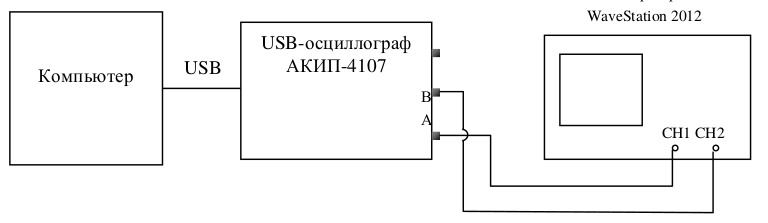
\includegraphics[width = 12cm, height = 5cm]{image1.png}
	\caption{Схема экспериментальной установки}
\end{figure}
\par
	Схема экспериментальной установки приведена на рис.1. Функциональный генератор WaveStation 2012 позволяет сформировать два различных электрических сигнала, которые выводятся на два независимых канала CH1 и CH2. Сигнал с канала CH1 подаётся на вход A, а сигнал с канала CH2 подаётся на вход B USB-осциллографа. Затем эти сигналы подаются на вход компьютера через USB-соединение. При работе USB-осциллографа в режиме осциллографа, на экране компьютера можно наблюдать каждый из сигналов в отдельности, а также их произведение. В режиме спектроанализатора можно наблюдать спектры этих сигналов.

\section*{Исследование спектра периодической последовательности прямоугольных импульсов} 
\begin{enumerate}
	\item
		На генераторе установим разность максимального и минимального значений сигнала равной $1$ В, смещение сигнала равным $0.5$ В, частоту повторения импульсов $f_\text{повт} = 1$ кГц, а длительность импульса $\tau = 100$ мкс.
	\item
		Проанализируем, как меняется спектр: при увеличении $\tau$ вдвое при неизменной частоте $f_\text{повт} = 1$ кГц и при увеличении $f_\text{повт}$ вдвое при неизменном $\tau = 100$ мкс.		
		\begin{figure}[h!]
			\centering
			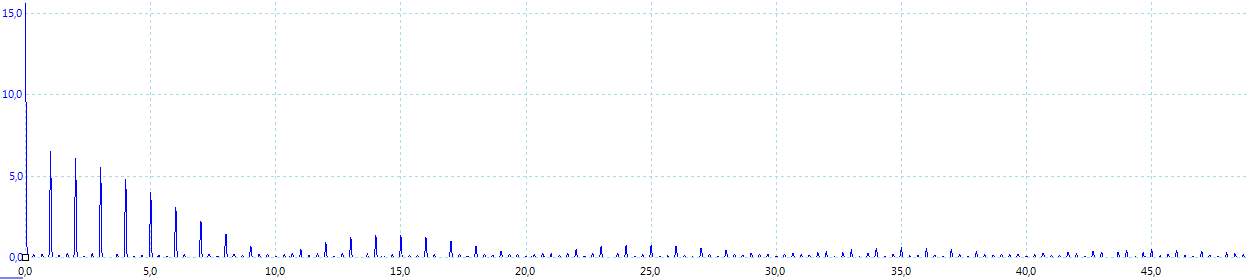
\includegraphics[width = 14cm, height = 4.8cm]{image2.png}
			\caption{Спектр сигнала при $f_\text{повт} = 1$ кГц и $\tau = 100$ мкс}			
		\end{figure}
		\begin{figure}[h!]
			\centering
			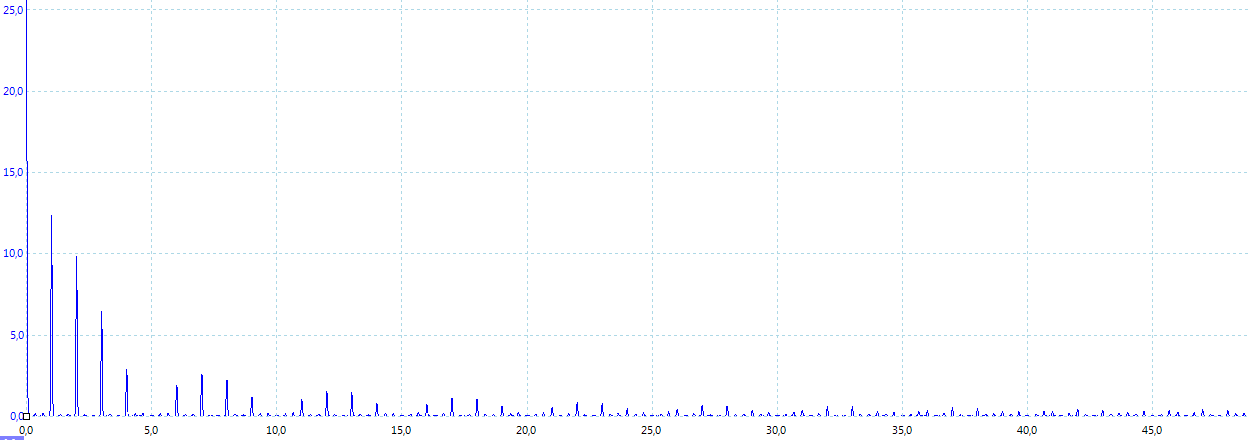
\includegraphics[width = 14cm, height = 4.8cm]{image3.png}
			\caption{Спектр сигнала при $f_\text{повт} = 1$ кГц и $\tau = 200$ мкс}			
		\end{figure}
		\newpage
		\begin{figure}[h!]
			\centering
			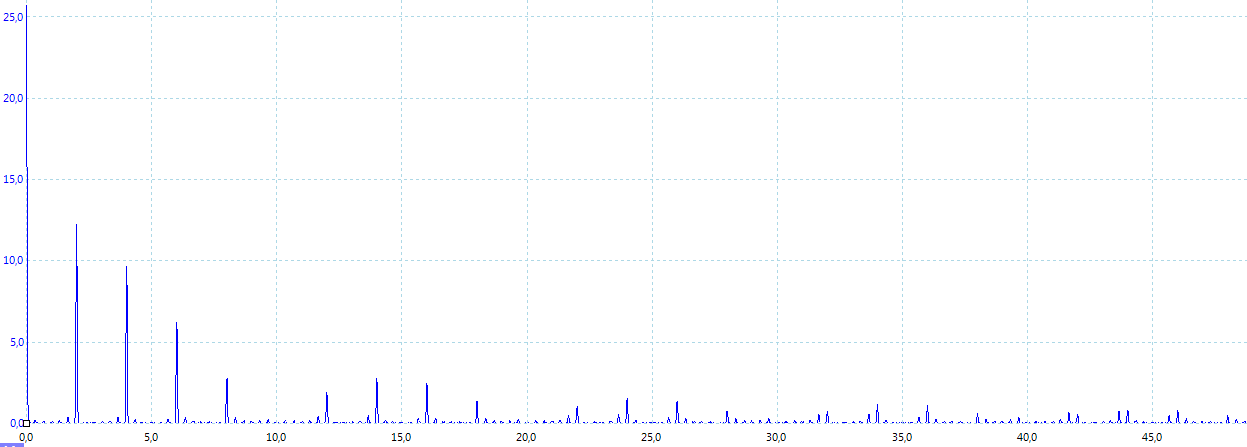
\includegraphics[width = 14cm, height = 4.8cm]{image4.png}
			\caption{Спектр сигнала при $f_\text{повт} = 2$ кГц и $\tau = 100$ мкс}			
		\end{figure}
	\item
		Проведём измерения ширины спектра $\Delta \nu$ от длительности импульса $\tau$ при увеличении $\tau$ от 40 до 200 мкс при $f_\text{повт} = 1$ кГц.
		\begin{table}[h!]
			\centering
			\begin{tabular}{|c|c|}
			\hline
				$\tau$, мкс & $\Delta \nu$, кГц \\
			\hline
				40 & 25.0 \\
			\hline
				50 & 20.0 \\
			\hline
				60 & 17.0 \\
			\hline
				70 & 14.0 \\
			\hline
				80 & 12.5 \\
			\hline
				120 & 8.5 \\
			\hline
				150 & 7.0 \\
			\hline
				200 & 5.0 \\
			\hline
			\end{tabular}
		\end{table}
	\par
		Построем график зависимости $\Delta \nu = 1 / \tau$ и по его наклону убедимся в справедливости соотношения неопределённостей ($\Delta \nu \Delta t \simeq 1$), что мы уже в принципе можем сделать, анализируя полученные измерения в таблице.
	\begin{figure}[h!]
		\centering
		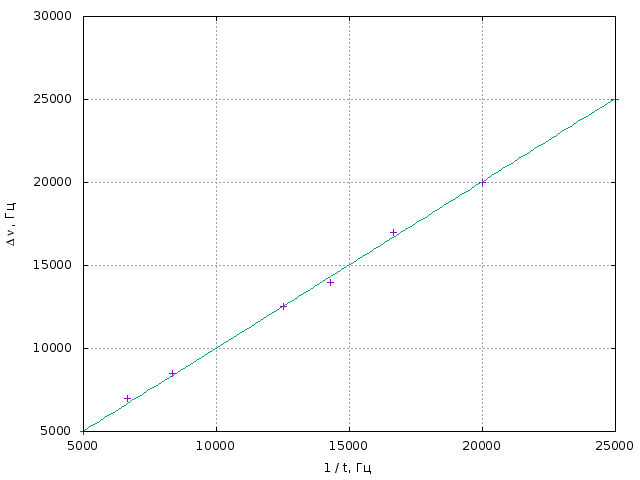
\includegraphics[width = 11cm, height = 6cm]{plot1.png}
		\caption{График зависимости $\Delta \nu = f(1 / \tau)$}
	\end{figure}	
	\par
		Коэффицент наклона		
	\[
		k = \left(1.003 \pm 0.005\right)
	\]
	\item
		Для $f_\text{повт} = 1$ кГц и $\tau = 50$ мкс и $\tau = 100$ мкс измерим частоты и амплитуды спектральных составляющих сигнала и занесём результаты в таблицу, где $N$ --- номер гармоники, $f$ --- частота, а $A$ --- амлитуда.
		\begin{table}[h!]
			\centering
			\begin{tabular}{|c|c|c|}
			\hline
				$N$ & $f$, кГц & $A$, мВ \\
			\hline
				2 & 2.016 & 102.1 \\
			\hline
				3 & 3.015 & 100.6 \\
			\hline
				4 & 3.993 & 99.1 \\
			\hline
				5 & 4.992 & 93.2 \\
			\hline
				6 & 6.011 & 85.8 \\
			\hline
				7 & 6.968 & 81.7 \\
			\hline
				8 & 8.028 & 72.5 \\
			\hline
				9 & 9.006 & 66.6 \\
			\hline
				10 & 9.964 & 62.13 \\
			\hline
			\end{tabular}
			\caption*{Измерения при $f_\text{повт} = 1$ кГц и $\tau = 50$ мкс}			
		\end{table}
		\begin{table}[h!]
			\centering
			\begin{tabular}{|c|c|c|}
			\hline
				$N$ & $f$, кГц & $A$, мВ \\
			\hline
				1 & 0.997 & 211.5 \\
			\hline
				2 & 1.996 & 199.7 \\
			\hline
				3 & 2.994 & 177.5 \\
			\hline
				4 & 3.973 & 158.3 \\
			\hline
				5 & 5.032 & 130.2 \\
			\hline
				6 & 5.990 & 102.1 \\
			\hline
				7 & 7.009 & 74.0 \\
			\hline
				8 & 7.986 & 45.9 \\
			\hline
				9 & 9.006 & 20.7 \\
			\hline
			\end{tabular}
			\caption*{Измерения при $f_\text{повт} = 1$ кГц и $\tau = 100$ мкс}			
		\end{table}
\end{enumerate}
\section*{Исследование спектра периодической последовательности цугов гармонических колебаний}
\begin{enumerate}
	\item
		Сделав все необходимые настройки в программе, проанализуем, как изменяется вид спектра для произведения $A * B$ при увеличении длительности $\tau$ импульса от 100 до 200 мкс.
		\begin{figure}[h!]
			\centering
			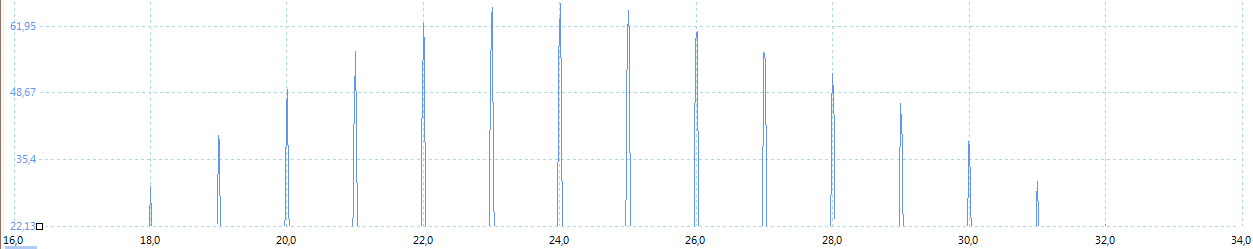
\includegraphics[width = 12cm, height = 6 cm]{image5.png}
			\caption{Спектр сигнала при $f_\text{повт} = 1$ кГц и $\tau = 100$ мкс}
		\end{figure}
		\begin{figure}[h!]
			\centering
			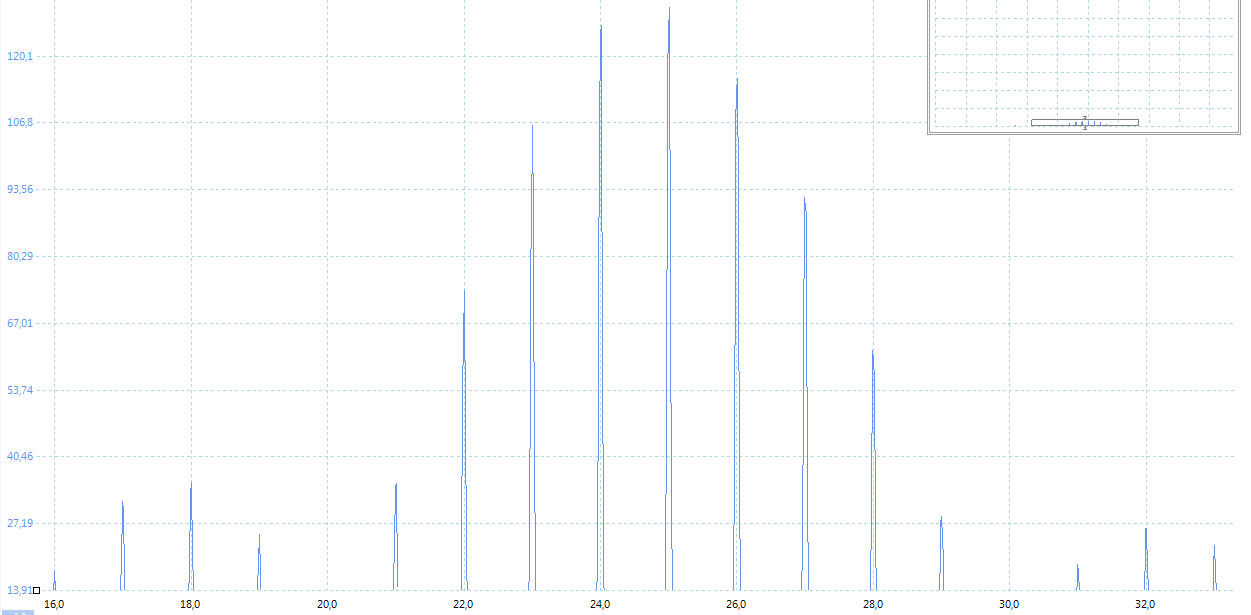
\includegraphics[width = 12cm, height = 6 cm]{image6.png}
			\caption{Спектр сигнала при $f_\text{повт} = 1$ кГц и $\tau = 200$ мкс}
		\end{figure} 
	\item
		Установив длительность импульса $\tau = 100$ мкс, проследим, как меняется картина спектра при изменении несущей частоты $\nu_0$ ($\nu_0 = 10, 25 и 40$ кГц).
		\begin{figure}[h!]
			\centering
			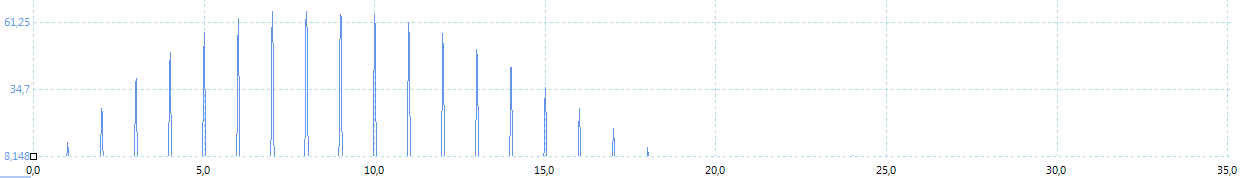
\includegraphics[width = 14cm, height = 5cm]{image7.png}
			\caption{Спектр сигнала при $\nu_0 = 10$ кГц и $\tau = 100$ мкс}
		\end{figure}
		\newpage
		\begin{figure}[h!]
			\centering
			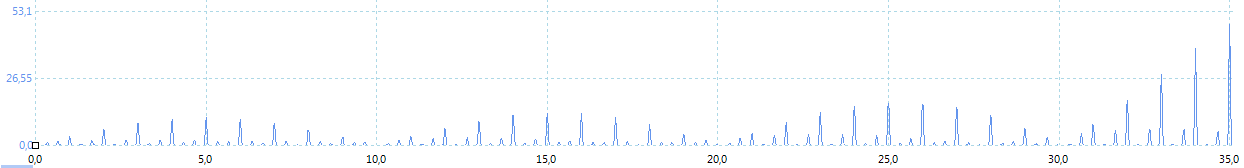
\includegraphics[width = 14cm, height = 5cm]{image8.png}
			\caption{Спектр сигнала при $\nu_0 = 25$ кГц и $\tau = 100$ мкс}
		\end{figure}
		\begin{figure}[h!]
			\centering
			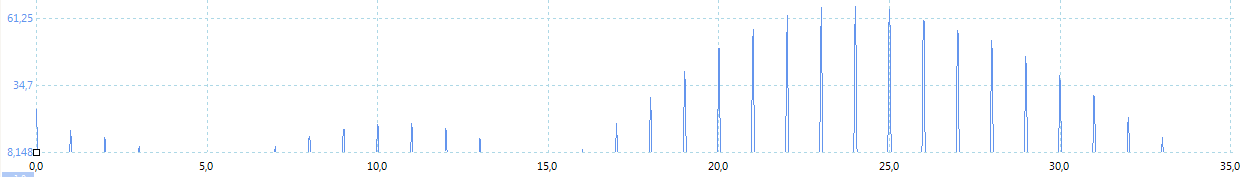
\includegraphics[width = 14cm, height = 5cm]{image9.png}
			\caption{Спектр сигнала при $\nu_0 = 40$ кГц и $\tau = 100$ мкс}
		\end{figure}
	\item
		Установим частоту несущей $\nu_0 = 30$ кГц и длительность импульса $\tau = 100$ мкс. Определим расстоние $\delta \nu$ между соседними спектральными компонентами для разных частот повторения импульса $f_\text{повт}$ ($f_\text{повт} = 0.5, 1, 2, 4, 5$ кГц)
		\begin{table}[h!]
			\centering
			\begin{tabular}{|c|c|}
			\hline
				$f_\text{повт}$, кГц & $\delta v$, кГц \\
			\hline
				0.5 & 0.48 \\
			\hline
				1 & 0.98 \\
			\hline
				2 & 1.99 \\
			\hline
				4 & 4.00 \\
			\hline
				5 & 5.01 \\ 
			\hline
			\end{tabular}		
		\end{table}
	\par
		Построим график $\delta \nu = g(f_\text{повт})$ (рис.11) и найдём угловой коэффициент полученной зависимости.
		\begin{figure}[h!]
			\centering
			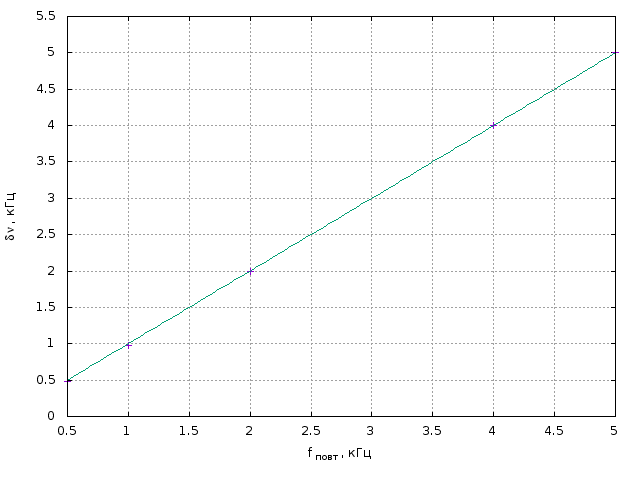
\includegraphics[width = 12cm, height = 7cm]{plot2.png}
			\caption{График зависимости $\delta \nu = g(f_\text{повт})$}
		\end{figure}
	\par
		В результате получим, что угловой коэффициент:
		\[
			k = \left(1.000 \pm 0.002\right)
		\]
	\item
		Установим $\tau = 100$ мкс и $f_\text{повт} = 1$ кГц. Определим амплитуды и частоты для различных гармоник при $f_\text{повт} \text{ равной } 1 \text{ и }2$ кГц и занесём результаты в таблицу, где $N$ --- номер гармоники, $f$ --- частота, а $A$ --- амлитуда.
		\begin{table}[h!]
			\centering
			\begin{tabular}{|c|c|c|}
			\hline
				$N$ & $f$, кГц & $A$, мВ \\
			\hline
				1 & 1 & 4.57 \\
			\hline
				2 & 2 & 8.74 \\
			\hline
				3 & 3 & 12.02 \\
			\hline
				4 & 4 & 13.91 \\
			\hline
				5 & 5 & 15.00 \\
			\hline
				11 & 11 &  4.67 \\
			\hline
				15 & 15 & 19.57 \\
			\hline
				25 & 25 & 44.71 \\
			\hline			
			\end{tabular}
			\caption*{Измерения при $f_\text{повт} = 1$ кГц и $\tau = 100$ мкс}
		\end{table}
		\begin{table}[h!]
			\centering
			\begin{tabular}{|c|c|c|}
			\hline
				$N$ & $f$, кГц & $A$, мВ \\
			\hline
				1 & 2 & 15.1 \\
			\hline
				2 & 4 & 28.12 \\
			\hline
				6 & 12 & 19.67 \\
			\hline
				7 & 14 & 35.57 \\
			\hline
				11 & 22 & 36.76 \\
			\hline
				12 & 24 &  74.10 \\
			\hline
				13 & 26 & 102.10 \\
			\hline			
			\end{tabular}
			\caption*{Измерения при $f_\text{повт} = 2$ кГц и $\tau = 100$ мкс}
		\end{table}
\end{enumerate}
\section*{Исследование спектра гармонических колебаний, модулированных по амлитуде}
\begin{enumerate}
	\item
	\par
		Для канала CH2 на генераторе установим двойную амплитуду сигнала равной 1 В, частоту несущей $\nu_0$ равной 25 кГц, также установим смещение сигнала равным нулю.
	\par
		Для канала CH1 на генераторе установим двойную амплитуду сигнала равной 0.2 В и частоту модуляции $f_\text{мод}$ равной 1 кГц. Смещение сигнала установим равным 1 В.
	\item
		Меняя двойную амплитуду сигнала канала CH1 от 0.2 до 2, измерим для каждого значения максимальную $A_\text{max}$ и $A_\text{min}$ амплитуды сигналов модулированного колебания и амплитуды спектральных компонент. Рассчитаем соответствующие значения глубины модуляции $m$ по формуле
		\[
			m = \frac{A_\text{max} - A_\text{min}}{A_\text{max} + A_\text{min}}
		\]
		\begin{table}[h!]
			\centering
			\begin{tabular}{|c|c|c|c|c|c|}
			\hline
				$2U$, В & $A_\text{min}$, мВ & $A_\text{max}$, мВ & $a_\text{осн}$, мВ & $a_\text{бок}$, мВ & $m$\\
			\hline
				0.2	& 430.5	& 548.6	& 322.3	& 40.6 & 0.12 \\
			\hline
				0.5	& 361.5	& 617.5	& 322.3	& 65.0 & 0.26 \\
			\hline
				0.8	& 278.0 & 691.3 & 322.3 & 97.4 & 0.43 \\
			\hline
				1.2	& 189.4 & 784.7 & 322.3 & 131.0 & 0.61 \\
			\hline
				1.6	& 95.9  & 893.0	& 322.3	& 170.0 & 0.81 \\
			\hline
			\end{tabular}
		\end{table}
	\par
		Построим график отношения $a_\text{бок} / a_\text{осн}$ в зависимости от $m$ (рис.12) и определим угловой коэффициент наклона графика.
		\newpage
		\begin{figure}[h!]
			\centering
			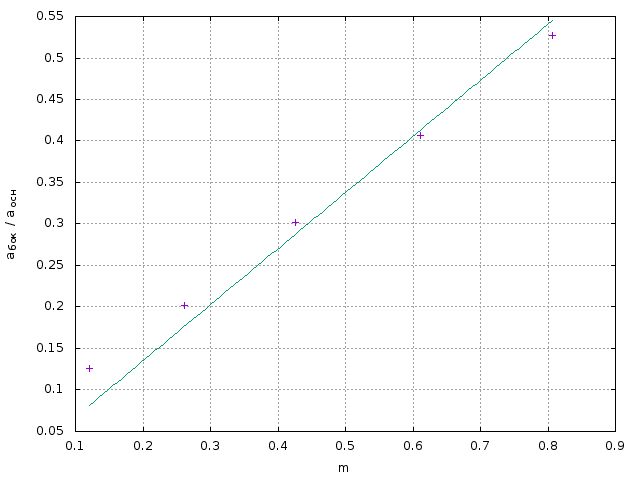
\includegraphics[width = 12cm, height = 6cm]{plot3.png}
			\caption{График зависимости $a_\text{бок} / a_\text{осн}$ от $m$}
		\end{figure}
		\par
		Угловой коэффициент наклона графика
		\[
			k = \left(0.68 \pm 0.03\right)
		\]
\end{enumerate}

\end{document}